Preamp boards have four digital inputs to set their mode for measurement or stimulation.  More experimentation is needed determine optimal relative timing of these inputs~\cite{StahlMSEE}.  The RTSC must have the ability to uniquely control each Preamp digital input, which means, for eight Preamp boards, a total of 32 external IO pins would be required of the Xilinx\textsuperscript{\textregistered} XC3S500E FPGA.  The Hirose FX2 connector on the RTSC exposes 40 IO pins, but many of those are needed for the DAC and ADC interfaces.  Thus, a CPLD provided on the Electrophysiology Interface board, as shown in Figure~\ref{fig:CPLD}, can act as an IO expander allowing the FPGA individual control of the four digital inputs on each of the eight Preamps connected to the Electrophysiology Interface board.

\begin{figure}[H]
	\centering 
		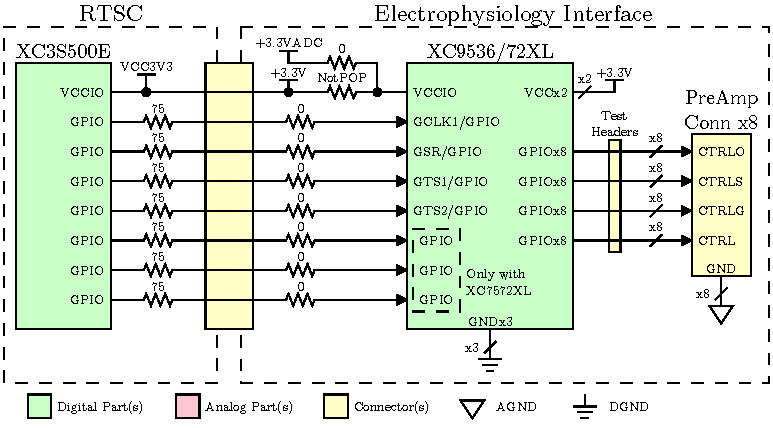
\includegraphics{./figures/CPLD} 
	\caption{Connections between the FPGA on the RTSC board and the CPLD and Preamp Connectors on the Electrophysiology Interface board\label{fig:CPLD}}
\end{figure}

A CPLD solves the problem of scarce IO very well.  The configuration of the CPLD can be changed based on the needs of the system as determined by experimentation: it could be configured to simply change all of the IO pins based on a single input, or it could be configured to respond to a complex serial interface with multiple commands and a clock input.  The XC9500XL series are Xilinx\textsuperscript{\textregistered} CPLD devices that have adequate number of IO pins available, that can be powered with a single $3.3\unit{V}$ voltage supply available on the Electrophysiology Interface board from the RTSC board, that retain their configuration between power cycles, and that use the same tools from Xilinx\textsuperscript{\textregistered} and Digilent\textsuperscript{\textregistered} for configuration, development, and programming as the FGPA on the RTSC board~\cite{XC9500XLds}.

The CPLD used must have enough external IO pins to connect to the eight Preamp boards plus a few IO pins for the interface with the FPGA.  The DAC and ADC use 33 of the 40 available FPGA IO connections leaving seven IO connections for the FPGA to CPLD interface.  Several package options are available for XC9500XL family, but the Quad Flat Pack (xQFP) variations offer the most flexibility in available parts and are relatively easy to solder by hand.  The 44-pin VQFP package offers only 34 external IO pins, which, after connecting the Preamp signals, leaves only 2 pins for the FPGA interface, but the 64-pin VQFP package offers 36 IO pins with the XC9536XL and 52 IO pins with the XC9572XL~\cite{DesignXC9500XLappnote}.  Designing the Electrophysiology Interface board for the XC9572XL in the 64-pin VQFP package will allow the XC9536XL to be used in its place for a cheaper price and lower power consumption, if the extra IO and logic gates offered by the XC9572XL are not needed.  A summary of the capabilities of the XC9536XL versus the XC9572XL on the Electrophysiology Interface board are shown in Table~\ref{tab:CPLDMigration}, which has information from~\cite{XC9500XLds} and~\cite{DesignXC9500XLappnote}.

\renewcommand{\arraystretch}{1.3}
\begin{table}[h]
\centering 
\begin{tabular}{|l|l|l|l|l|l|}

\hline
CPLD	& IO Pins & Macrocells & Gates & Preamp Signals & FPGA Signals\\
\hline
XC9536XL	& 36 & 36 & 800 & 32 & 4\\
\hline
XC9572XL	& 52 & 72 & 1600 & 32 & 7\\
\hline
\end{tabular}
\caption{XC9536XL and XC9572XL VQFP-64 capabilities on the Electrophysiology Interface board~\cite{XC9500XLds,DesignXC9500XLappnote}\label{tab:CPLDMigration} }

\end{table}
\renewcommand{\arraystretch}{1.0}

Four of the signals from the FPGA are connected to special function pins of the CPLD.  These pins provide low-latency operation for the special functions, but may be configured as general purpose IO (GPIO), if the special functions aren't needed.

Test headers provide access to the signals between the CPLD and the Preamp connectors.  There are two internal power supply pins, VCC, that are connected to the $+3.3\unit{V}$ power rail that is connected to the VCC3V3 power supply on the RTSC board.  There is a separate power supply input pin for the IO buffers, VCCIO, that can be connected to $+3.3\unit{V}$ or to the output of the $3.3\unit{V}$ regulator on the Electrophysiology Interface board, labeled as $+3.3\unit{VADC}$.  VCCIO and VCC can be powered in any sequence without harming the part~\cite{DesignXC9500XLappnote}.

The digital inputs on the Preamp boards are connected to an Analog Devices ADG202A quad analog switch IC.  Its digital input requirements are compared to the digital output specifications of the XC9536XL and XC9572XL, with $\mathrm{VCCIO}=3.3\unit{V}$, in Table~\ref{tab:PreampCPLDVolt}, which shows that the CPLD outputs are compatible with the ADG202A inputs~\cite{ADG202Ads,XC9536XLds,XC9572XLds}.

\renewcommand{\arraystretch}{1.3}
\begin{table}[h]
\centering 
\begin{tabular}{|l|l|l|}
\hline
Logic	& HIGH & LOW\\
\hline
ADG202A	Input & $2.4\unit{Vmin}$ & $0.8\unit{Vmax}$\\
\hline
XC9536/72XL	Output & $2.4\unit{Vmin}$ & $0.4\unit{Vmax}$\\
\hline
\end{tabular}
\caption{AD202A quad analog switch and XC9536/72XL CPLD digital input and output compatibility\label{tab:PreampCPLDVolt} }

\end{table}
\renewcommand{\arraystretch}{1.0}

One possible situation that might cause damage to the CPLD when connected to the Preamp Board is the connection of the digital inputs on the Preamp Board to the analog voltage supplies.  The XC9536XL and XC9572XL have a maximum rating on its input and three-state output pins of $5.5\unit{V}$~\cite{XC9536XLds,XC9572XLds}.  If the Preamp board ties a digital input to its positive analog voltage supply, the voltage on the CPLD pins could exceed their maximum rating.  Tieing the digital inputs on the Preamp boards to a HIGH logic level should be accomplished with a voltage divider to ensure that the maximum voltage does not exceed $5.5\unit{V}$.
